%%%%%%%%%%%%%%%%%%%%%%%%%%%%%%%%%%%%%%%%%%%%%%%%%%%%%%%%%%%
% --------------------------------------------------------
%  _____           
% |_   _|_ _ _   _ 
%   | |/ _` | | | |
%   | | (_| | |_| |
%   |_|\__,_|\__,_|
%
% LaTeX2e Template
% Version 2.6.0 (21/04/2026)
%
% Author: 
% Guillermo Jimenez (memo.notess1@gmail.com)
% 
% License:
% Creative Commons CC BY 4.0
% --------------------------------------------------------
%%%%%%%%%%%%%%%%%%%%%%%%%%%%%%%%%%%%%%%%%%%%%%%%%%%%%%%%%%%
% --------------------------------------------------------
% Github Repository:
% https://github.com/MemoJimenez/Tau-class
% --------------------------------------------------------
%%%%%%%%%%%%%%%%%%%%%%%%%%%%%%%%%%%%%%%%%%%%%%%%%%%%%%%%%%%

\documentclass[9pt,a4paper,twocolumn,twoside]{tau-class/tau}
\usepackage[utf8]{inputenc} %inserisco per utf8 code
\usepackage[T1]{fontenc}
\usepackage[italian]{babel} %ci proviamo per italiano

% Spanish babel recomendation
% \usepackage[spanish,es-nodecimaldot,es-noindentfirst]{babel} 

%----------------------------------------------------------
% Title & Authors/Affiliations
%----------------------------------------------------------

\doctype{Report Data Science}
\title{Previsione dell'Abbandono dei Dipendenti (Employee Attrition)}

%----------------------------------------------------------

\author[a,1]{Paolo Magnanelli\thanks{\href{mailto:paolo.magnanelli@studio.unibo.it}{paolo.magnanelli@studio.unibo.it} (P. Magnanelli)}}
\author[a,2]{Asia Milan\thanks{\href{mailto:asia.milan@@studio.unibo.it}{asia.milan@@studio.unibo.it} (A. Milan)}}

%----------------------------------------------------------

\affil[a]{Università di Bologna}

%----------------------------------------------------------
% Document-, Footer- information
%----------------------------------------------------------

\dates{Questo report è stato redatto il \today}

%----------------------------------------------------------

\footinfo{Introduzione alla Data Science e al Pensiero Computazionale}
\theday{\today}
\organization{Università di Bologna}
\leadauthor{P. Magnanelli e A. Milan}

%----------------------------------------------------------
% Abstract and Keywords
%----------------------------------------------------------

\begin{abstract}
Questo lavoro presenta un'analisi esplorativa e predittiva del fenomeno dell'\emph{attrition} (abbandono dei dipendenti) a partire dal dataset \textit{Employee Attrition}. Dopo una fase di comprensione e pulizia dei dati, viene condotta un'analisi esplorativa multivariata per identificare i fattori associati all'abbandono, seguita dall'addestramento e dal confronto di tre modelli di classificazione (regressione logistica, k-Nearest Neighbors e Random Forest). I risultati mostrano che variabili come straordinari (\texttt{OverTime}), reddito mensile ed età sono fortemente associate all'attrition, e che la regressione logistica ottiene le prestazioni migliori in termini di \emph{recall} sulla classe minoritaria e di area sotto la curva ROC (AUC), risultando inoltre il modello più interpretabile.
\end{abstract}

%----------------------------------------------------------

\keywords{Regressione Logistica, K-NN, Random Forest, Employee Attrition}

%----------------------------------------------------------

\begin{document}
		
    \maketitle 
    \thispagestyle{firststyle}
    
%----------------------------------------------------------

\begin{note}
    In conformtità alla licenza CC BY 4.0, questo template è stato creato da Guillermo Jimenez (memo.notess1@gmail.com)
\end{note}

%----------------------------------------------------------
\section{Introduzione}
\taustart{L}'abbandono volontario dei dipendenti (\emph{employee attrition}) rappresenta uno dei problemi più rilevanti nella gestione delle risorse umane: ogni dimissione comporta costi diretti (selezione, assunzione, formazione) e indiretti (perdita di know-how, impatto sul morale del team), che la letteratura manageriale stima in una quota significativa della retribuzione
annua del dipendente che lascia l'azienda \cite{allen2010retention}.

\subsection{obbiettivo}
L'obiettivo di questo progetto è duplice. Da un lato, si vuole comprendere \emph{quali} fattori organizzativi, demografici ed economici sono più associati alla decisione di un dipendente di lasciare l'azienda, attraverso un'analisi esplorativa dei dati (Sezioni~\ref{sec:metodologia} e \ref{sec:risultati}). Dall'altro, si vuole costruire un modello predittivo in grado di stimare la probabilità di abbandono di un dipendente, confrontando tre approcci di classificazione supervisionata con caratteristiche diverse: un modello lineare e interpretabile (regressione logistica), un modello basato su distanza (k-NN) e un modello ad albero in ensemble (Random Forest).

\subsection{fasi del progetto}
Il progetto segue un percorso in fasi successive: comprensione del dataset, analisi esplorativa, modellazione, valutazione critica dei risultati e, in ultimo, alcuni approfondimenti su soglie decisionali e curve ROC/Precision-Recall. Il codice completo, comprensivo di tutte le celle di analisi e dei grafici riportati in questo documento, è disponibile nel repository GitHub del progetto (Sezione~\ref{sec:Github Repository}).

%----------------------------------------------------------
\section{Dataset}
\label{sec:dataset}

\taustart{I}l dataset utilizzato è \textit{Employee Attrition}, un dataset sintetico ampiamente utilizzato in ambito didattico per problemi di classificazione in ambito HR \cite{ibm_hr_attrition}. Esso contiene $1470$ osservazioni, ciascuna corrispondente a un dipendente, descritte da $35$ variabili.

Le variabili si dividono in $26$ numeriche (ad esempio \texttt{Age}, \texttt{MonthlyIncome}, \texttt{TotalWorkingYears}, \texttt{YearsAtCompany}) e $9$ categoriche (tra cui \texttt{Department}, \texttt{JobRole}, \texttt{MaritalStatus}, \texttt{BusinessTravel}, \texttt{OverTime} e la variabile target \texttt{Attrition}). Non sono presenti valori mancanti in nessuna delle colonne.

Tre variabili numeriche (\texttt{EmployeeCount}, \texttt{Over18},
\texttt{StandardHours}) assumono un unico valore costante per tutte le osservazioni e sono pertanto non informative; sono state escluse, insieme all'identificativo \texttt{EmployeeNumber}, dalla fase di modellazione.

\begin{table}[ht]
    \centering
    \begin{tabular}{lcc}
        \toprule
        \textbf{Attrition} & \textbf{Numero} & \textbf{ in Percentuale (\%)} \\
        \midrule
        No  & 1233 & 83.88 \\
        Yes & 237  & 16.12 \\
        \bottomrule
    \end{tabular}
    \caption{Distribuzione di Attrition: conteggi e percentuali.}
    \label{tab:attrition-counts}
\end{table}


La variabile target \texttt{Attrition} è binaria (\texttt{Yes}/\texttt{No}) e risulta fortemente sbilanciata, come mostrato nella tabella ~\ref{tab:attrition-counts}: circa l'84\% dei dipendenti resta in azienda, mentre solo il 16\% circa lascia. Questo sbilanciamento ha conseguenze rilevanti sia sulla scelta delle metriche di valutazione (la sola \emph{accuracy} risulta poco informativa, si veda la Sezione~\ref{sec:risultati}), sia sulla strategia di addestramento dei modelli, per i quali è stata utilizzata una suddivisione \emph{stratificata} tra train e test.

\begin{figure}[ht]
    \centering
    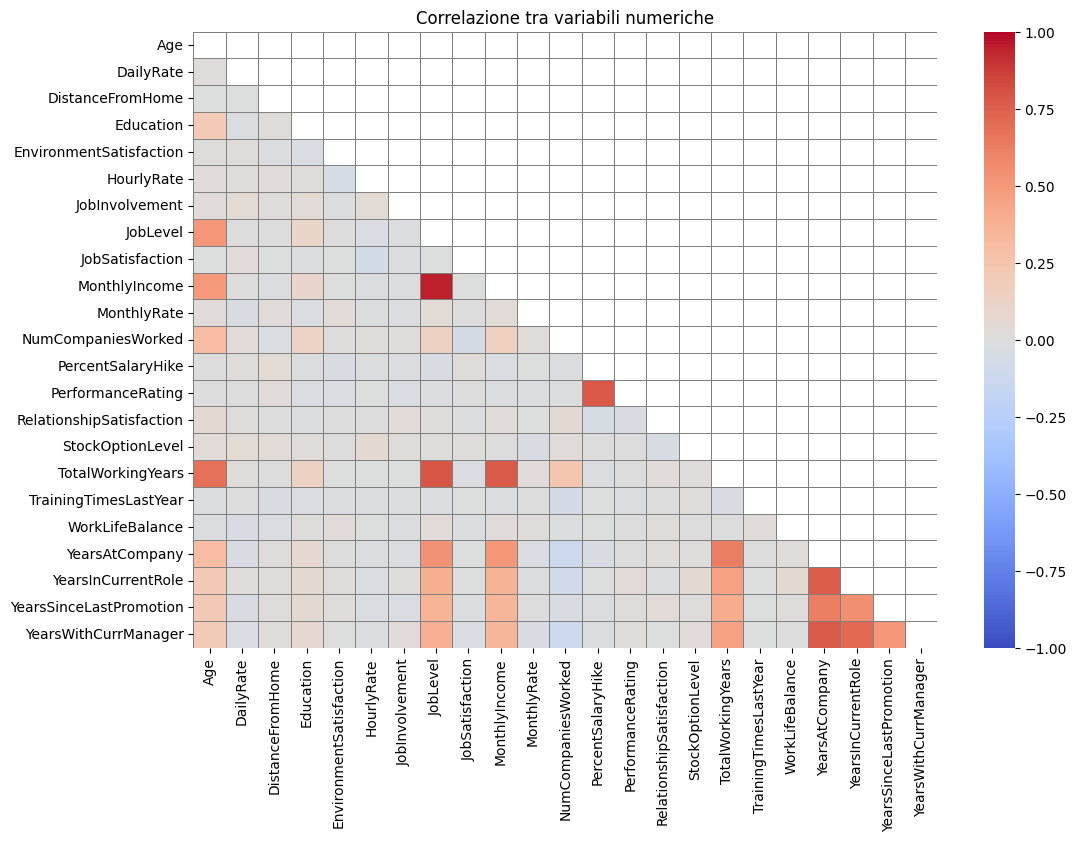
\includegraphics[width=\columnwidth]{figures/fase2_domanda8_correlazione.png}
    \caption{Matrice di correlazione tra le variabili numeriche del dataset (Fase 2, Domanda 8).}
    \label{fig:correlazione}
\end{figure}

L'analisi delle correlazioni tra le variabili numeriche (Figura~\ref{fig:correlazione}) evidenzia alcune relazioni attese: una correlazione molto elevata tra \texttt{JobLevel} e \texttt{MonthlyIncome}, e correlazioni marcate tra le variabili legate all'anzianità in azienda (\texttt{YearsAtCompany}, \texttt{YearsInCurrentRole}, \texttt{YearsWithCurrManager}). Queste relazioni sono state tenute in considerazione nell'interpretazione dei coefficienti dei modelli in Sezione~\ref{sec:risultati}.

%----------------------------------------------------------
\section{Metodologia}
\label{sec:metodologia}

\subsection{Comprensione del dataset (Fase 2)}
\taustart{I}n questa fase è stata effettuata un'analisi descrittiva preliminare: verifica dei valori mancanti, identificazione delle variabili costanti, analisi della distribuzione della variabile target e calcolo delle statistiche descrittive (media, mediana, deviazione standard) per le variabili numeriche più rilevanti. È stata inoltre calcolata la matrice di correlazione tra tutte le variabili numeriche per individuare eventuali ridondanze.

\subsection{Analisi esplorativa e visualizzazione (Fase 3)}
Sono state formulate e analizzate diverse domande di ricerca, incrociando la variabile target con le principali variabili numeriche e categoriche: straordinari (\texttt{OverTime}), reddito mensile, ruolo lavorativo (\texttt{JobRole}), equilibrio vita lavoro (\texttt{WorkLifeBalance}), età ed esperienza in azienda, numero di aziende precedenti e anzianità lavorativa complessiva. Per ciascuna domanda sono stati prodotti grafici dedicati (boxplot, barplot, heatmap, scatterplot) e formulate considerazioni quantitative.

\subsection{Modellazione (Fase 4)}
Dopo aver rimosso le colonne non informative (variabili costanti, \texttt{EmployeeNumber}, e la colonna ridondante \texttt{Attrition\_num} derivata dal target), le variabili categoriche sono state trasformate in variabili numeriche tramite \emph{one-hot encoding} con \texttt{pd.get\_dummies(..., drop\_first=True)}, per evitare collinearità perfetta tra le dummy generate. Il dataset così ottenuto è stato suddiviso in training (70\%) e test (30\%) tramite \texttt{train\_test\_split}, con stratificazione sulla variabile target per preservare le proporzioni delle classi in entrambi gli insiemi, e con \texttt{random\_state=42} per garantire la riproducibilità.

Le feature sono state standardizzate (media nulla, varianza unitaria) tramite \texttt{StandardScaler}, operazione necessaria per il k-NN, che si basa sulla distanza euclidea tra osservazioni, e comunque utile per migliorare la stabilità numerica della regressione logistica.

Sono stati addestrati tre modelli di classificazione con caratteristiche complementari, scelti per coprire approcci lineari, basati su distanza e ad albero \cite{hastie2009elements}:

\begin{itemize}
    \item \textbf{Regressione logistica}, modello lineare che stima la probabilità di appartenenza alla classe positiva (\texttt{Attrition = Yes}) come funzione logistica di una combinazione lineare delle feature;
    \item \textbf{k-Nearest Neighbors (k-NN)}, modello non parametrico che classifica ogni osservazione in base alla classe maggioritaria tra i $k$ vicini più prossimi nello spazio delle feature standardizzate. Il valore $k=14$ è stato scelto confrontando l'accuracy ottenuta al variare di $k\in \{1,3,5,7,9,11,14,18,21,35,51\}$ (Figura~\ref{fig:knn_k});
    \item \textbf{Random Forest} \cite{breiman2001random}, modello
    \emph{ensemble} composto da $200$ alberi di decisione, ciascuno
    addestrato su un sottoinsieme campionato con \emph{bootstrap} delle osservazioni e delle feature.
\end{itemize}

\begin{figure}[ht]
    \centering
    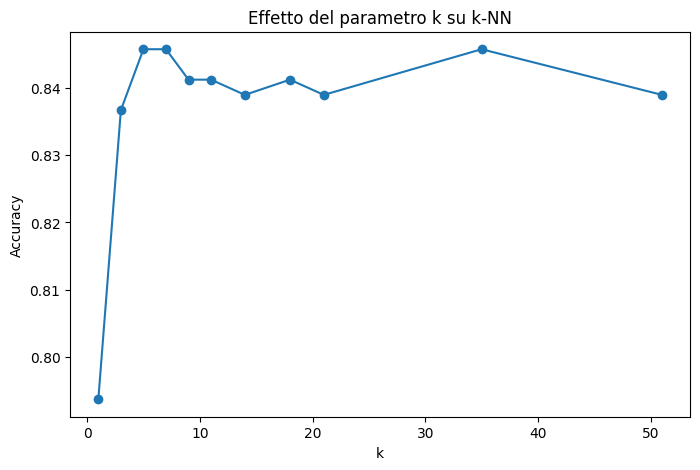
\includegraphics[width=\columnwidth]{figures/fase4_knn_accuracy_k.png}
    \caption{Accuracy del k-NN sul test set al variare del numero di vicini $k$ (Fase 4). Il valore $k=14$ è stato selezionato come compromesso tra accuracy e stabilità del modello.}
    \label{fig:knn_k}
\end{figure}

\subsubsection{La regressione logistica}
La regressione logistica modella la probabilità che un dipendente lasci l'azienda ($y=1$) condizionatamente al vettore di feature $\mathbf{x}$ tramite la funzione logistica (sigmoide) applicata a una combinazione lineare dei predittori:

\begin{equation}
P(y = 1 \mid \mathbf{x}) = \sigma(z)=\frac{1}{1+e^{-z}}
\label{eq:logistic}
\end{equation}

dove $\mathbf{w}$ è il vettore dei coefficienti del modello, $b$ è
l'intercetta e $\sigma(z)$ è la funzione sigmoide. I parametri
$\mathbf{w}$ e $b$ sono stimati per massimizzazione della verosimiglianza sui
dati di training. Una proprietà importante di questo modello, sfruttata nell'interpretazione dei risultati (Sezione~\ref{sec:risultati}), è che il segno e la magnitudine di ciascun coefficiente $w_i$ indicano rispettivamente la direzione e l'intensità dell'effetto della feature $x_i$ sul log-odds di abbandono, a parità delle altre variabili.

\subsection{Valutazione e interpretazione (Fase 5 e 5 bis)}
Le prestazioni dei tre modelli sono state confrontate sul test set
utilizzando \emph{accuracy}, \emph{precision}, \emph{recall} e
\emph{F1-score}, calcolate specificamente sulla classe minoritaria
(\texttt{Attrition = Yes}), data la natura sbilanciata del problema. Sono state inoltre prodotte le matrici di confusione per ciascun modello e analizzati, rispettivamente, i coefficienti standardizzati della regressione logistica e l'importanza delle feature (\emph{feature importance}) della Random Forest, per comprendere quali variabili pesano maggiormente nelle previsioni.

In un secondo approfondimento (Fase 5 bis) sono state calcolate le curve ROC e l'area sotto la curva (AUC) per i tre modelli, e la curva Precision-Recall per la regressione logistica al variare della soglia di decisione, per valutare il \emph{trade-off} tra precision e recall in funzione del contesto applicativo.

%----------------------------------------------------------
\section{Risultati}
\label{sec:risultati}

\subsection{Analisi esplorativa}

\taustart{L}'analisi esplorativa condotta in Fase 3 evidenzia diversi pattern
consistenti tra le variabili e l'attrition. In particolare, lo svolgimento di straordinari (\texttt{OverTime}) risulta fortemente associato all'abbandono: come mostrato nella tabella ~\ref{tab:overtime-attrition},il tasso di attrition tra i dipendenti che fanno straordinari è di circa il 31\%, contro circa il 10\% tra chi non ne fa, un rapporto di circa tre volte.

\begin{table}[ht]
    \centering
    \begin{tabular}{lcc}
        \toprule
        \textbf{OverTime} & \textbf{No} & \textbf{Yes} \\
        \midrule
        No  & 89.56 & 10.44 \\
        Yes & 69.47 & 30.53 \\
        \bottomrule
    \end{tabular}
    \caption{Percentuali di Attrition per stato di OverTime.}
    \label{tab:overtime-attrition}
\end{table}


Anche l'equilibrio vita-lavoro (\texttt{WorkLifeBalance}) mostra una
relazione chiara con l'attrition: la percentuale di abbandono è più alta tra i dipendenti con un work-life balance scarso e diminuisce progressivamente al migliorare dell'equilibrio, stabilizzandosi tra i livelli ``buono'' e ``ottimo''.

L'analisi congiunta di età ed esperienza in azienda (Figura~\ref{fig:eta_esperienza}) mostra che il rischio di abbandono si concentra nelle fasi iniziali della carriera: tra i dipendenti più giovani (18--25 anni) e con minore esperienza (categoria ``Nuovi'') si osserva il valore di attrition più elevato, pari al 41,7\%. Il rischio diminuisce progressivamente sia con l'aumentare dell'età sia con l'aumentare dell'esperienza in azienda.

\begin{figure}[ht]
    \centering
    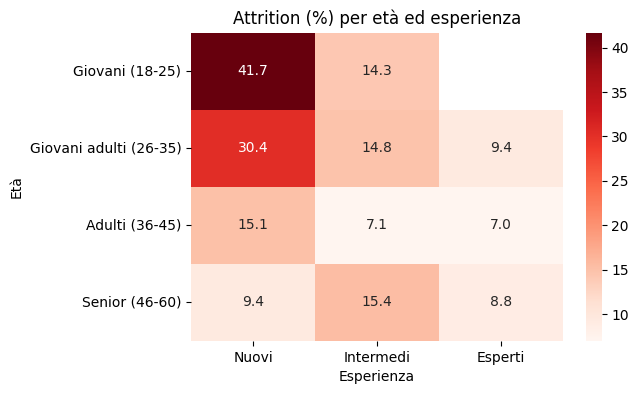
\includegraphics[width=\columnwidth]{figures/fase3_domanda5_eta_esperienza_heatmap.png}
    \caption{Percentuale di attrition per combinazione di fascia d'età ed esperienza in azienda (Fase 3, Domanda 5).}
    \label{fig:eta_esperienza}
\end{figure}

Il reddito mensile risulta più basso, in mediana, tra i dipendenti che lasciano l'azienda rispetto a chi resta, e questa differenza si mantiene \emph{all'interno} di ciascun ruolo lavorativo (\texttt{JobRole}), indicando che non si tratta semplicemente di un effetto di composizione tra ruoli diversi. Al contrario, il numero di aziende lavorate in precedenza (\texttt{NumCompaniesWorked}) non mostra una relazione evidente con l'attrition.

\subsection{Confronto tra modelli predittivi}
La Tabella~\ref{tab:metriche} riassume le metriche principali calcolate sul test set (441 osservazioni) per i tre modelli, con riferimento alla classe minoritaria \texttt{Attrition = Yes}.

\begin{table}[ht]
    \centering
    \caption{Confronto delle metriche di valutazione sul test set per la classe \texttt{Attrition = Yes}.}
    \label{tab:metriche}
    \begin{tabular}{lcccc}
        \toprule
        \textbf{Modello} & \textbf{Accuracy} & \textbf{Precision} & \textbf{Recall} & \textbf{F1-score} \\
        \midrule
        Regressione logistica & 0,875 & 0,690 & 0,408 & 0,513 \\
        k-NN ($k=14$)         & 0,839 & 0,500 & 0,056 & 0,101 \\
        Random Forest         & 0,832 & 0,429 & 0,127 & 0,196 \\
        Decision Tree         & 
        \bottomrule
    \end{tabular}
\end{table}

Come si osserva dalla Tabella~\ref{tab:metriche}, l'accuracy è simile e relativamente elevata per tutti i modelli (tra l'83\% e l'88\%), ma risulta una metrica poco informativa data la natura sbilanciata del dataset: un classificatore che predicesse sempre la classe maggioritaria \texttt{No} otterrebbe un'accuracy di circa l'84\% senza individuare correttamente alcun caso di abbandono. Guardando invece a precision, recall e F1-score sulla classe\texttt{Yes}, la regressione logistica risulta nettamente superiore agli altri due modelli, con una recall del 40,8\% contro il 5,6\% del k-NN e il 12,7\% della Random Forest.

%\begin{figure}[ht]
%    \centering
%   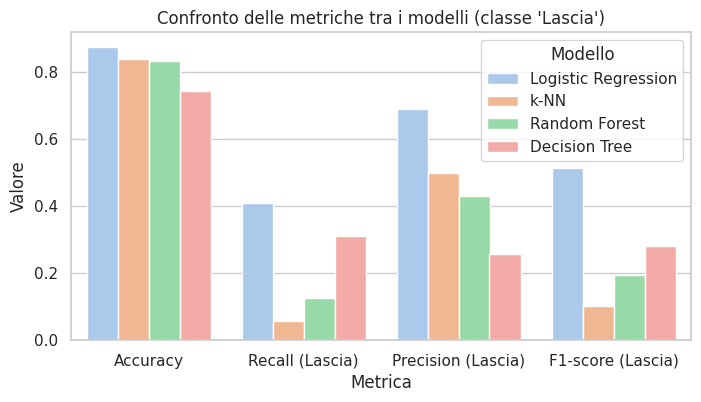
\includegraphics[width=\columnwidth]{figures/fase5_confronto_metriche_modelli.png}
%    \caption{Confronto delle metriche di valutazione tra i tre modelli, per la classe \texttt{Attrition = Yes} (Fase 5).}
%    \label{fig:confronto_metriche}
%\end{figure}

La matrice di confusione della regressione logistica (Figura~\ref{fig:confusion_logistica}) mostra che il modello classifica correttamente 357 dei 370 dipendenti che restano e 29 dei 71 che lasciano, con 42 falsi negativi e 13 falsi positivi. In tutti e tre i modelli, gli errori più frequenti sono falsi negativi (dipendenti a rischio non identificati), un tipo di errore particolarmente costoso in un contesto applicativo reale, perché impedisce di intervenire preventivamente su questi dipendenti.

\begin{figure}[ht]
    \centering
    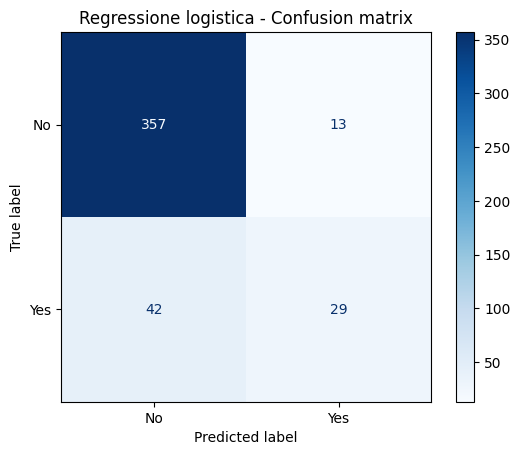
\includegraphics[width=\columnwidth]{figures/fase5_confusion_logistica.png}
    \caption{Matrice di confusione della regressione logistica sul test set (Fase 5).}
    \label{fig:confusion_logistica}
\end{figure}

L'analisi dei coefficienti standardizzati della regressione logistica (Figura~\ref{fig:coef_logistica}) mostra che la feature con il maggiore effetto positivo sulla probabilità di attrition è \texttt{OverTime\_Yes}, seguita da \texttt{BusinessTravel\_Travel\_Frequently} e da alcuni ruoli specifici. Tra gli effetti negativi più rilevanti figurano \texttt{TotalWorkingYears}, \texttt{EnvironmentSatisfaction} e \texttt{YearsInCurrentRole}, coerentemente con l'idea che maggiore esperienza e maggiore soddisfazione ambientale siano associate a una minore propensione all'abbandono.

\begin{figure}[ht]
    \centering
    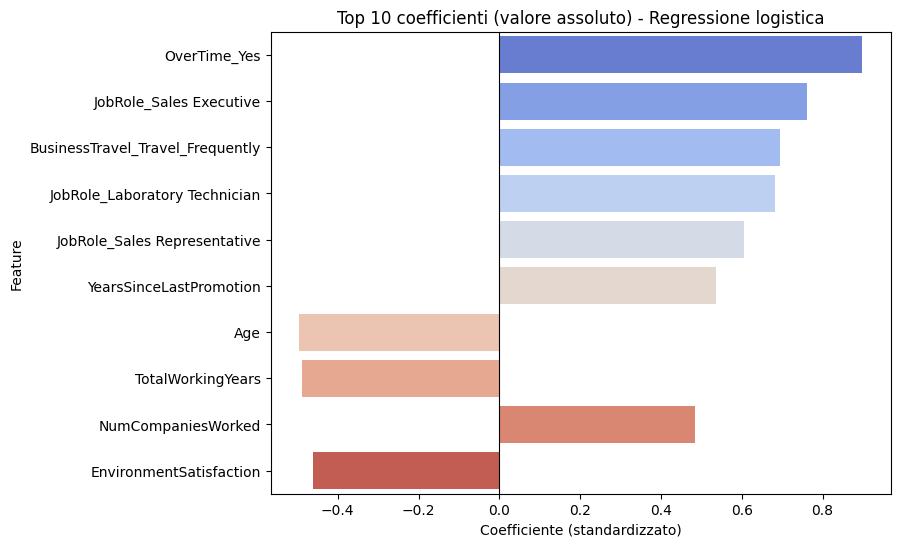
\includegraphics[width=\columnwidth]{figures/fase5_coefficienti_logistica.png}
    \caption{I 10 coefficienti (in valore assoluto) più rilevanti della regressione logistica, su feature standardizzate (Fase 5).}
    \label{fig:coef_logistica}
\end{figure}

La Random Forest, sebbene meno performante in termini di recall, fornisce un'indicazione complementare tramite la \emph{feature importance} (Figura~\ref{fig:feature_importance_rf}): le variabili più rilevanti risultano \texttt{MonthlyIncome}, \texttt{Age} e
\texttt{TotalWorkingYears}, in linea con quanto osservato sia nella
regressione logistica sia nell'analisi esplorativa di Fase 3.

\begin{figure}[ht]
    \centering
    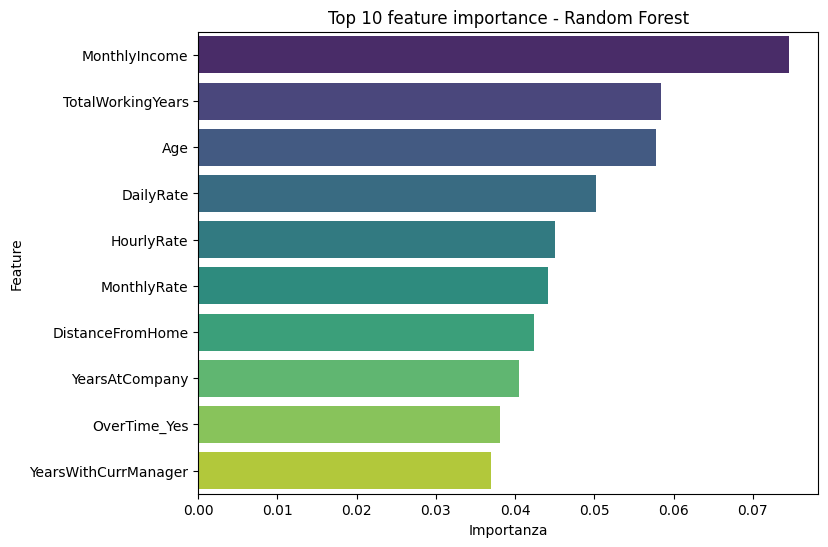
\includegraphics[width=\columnwidth]{figures/fase5_feature_importance_rf.png}
    \caption{Le 10 feature con maggiore importanza nella Random Forest (Fase 5).}
    \label{fig:feature_importance_rf}
\end{figure}

\subsection{Approfondimenti: curva ROC e soglia di decisione}

La curva ROC (Figura~\ref{fig:roc}) confronta i tre modelli a parità di soglia ideale, calcolando l'area sotto la curva (AUC). La regressione logistica ottiene l'AUC più alta (0,820), seguita dalla Random Forest (0,776) e dal k-NN (0,702). Questo risultato confema che la regressione logistica ordina meglio i dipendenti per rischio di attrition, anche al di là della soglia di decisione standard di 0,5 utilizzata nella Tabella~\ref{tab:metriche}.

\begin{figure}[ht]
    \centering
    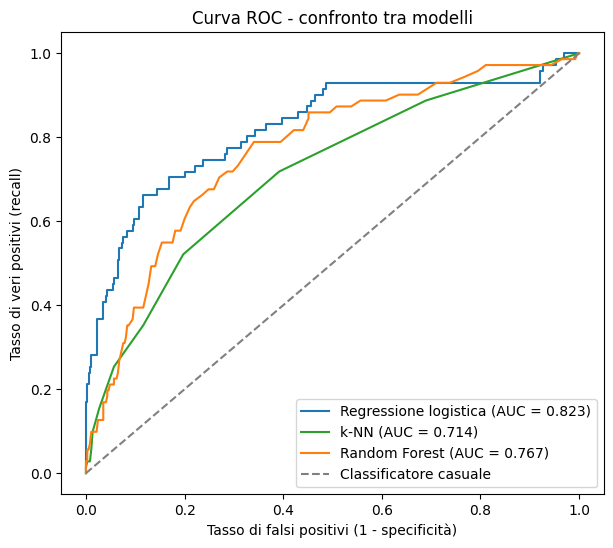
\includegraphics[width=\columnwidth]{figures/fase5bis_curva_roc.png}
    \caption{Curva ROC e AUC per i tre modelli (Fase 5 bis).}
    \label{fig:roc}
\end{figure}

Infine, la curva Precision-Recall per la regressione logistica
(Figura~\ref{fig:precision_recall}) mostra il \emph{trade-off} tra precision e recall al variare della soglia di decisione. La Tabella~\ref{tab:soglie} riporta i valori puntuali per alcune soglie selezionate: abbassando la soglia a 0,2--0,3 la recall sulla classe \texttt{Yes} aumenta sensibilmente rispetto alla soglia standard di 0,5, a costo di una precision più bassa.

\begin{figure}[ht]
    \centering
    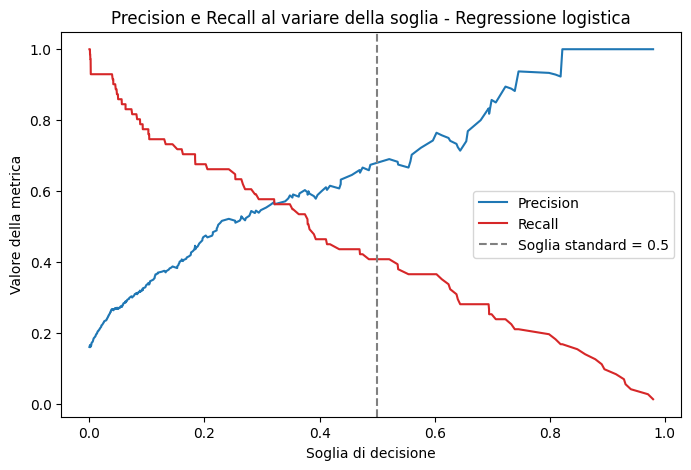
\includegraphics[width=\columnwidth]{figures/fase5bis_precision_recall.png}
    \caption{Curva Precision-Recall per la regressione logistica al variare della soglia di decisione (Fase 5 bis).}
    \label{fig:precision_recall}
\end{figure}

\begin{table}[ht]
    \centering
    \caption{Precision, recall e F1-score sulla classe \texttt{Attrition = Yes} per diverse soglie di decisione della regressione logistica.}
    \label{tab:soglie}
    \begin{tabular}{cccc}
        \toprule
        \textbf{Soglia} & \textbf{Precision} & \textbf{Recall} & \textbf{F1-score} \\
        \midrule
        0,2 & 0,448 & 0,662 & 0,534 \\
        0,3 & 0,526 & 0,563 & 0,544 \\
        0,4 & 0,660 & 0,493 & 0,565 \\
        0,5 & 0,725 & 0,408 & 0,523 \\
        0,7 & 0,889 & 0,225 & 0,360 \\
        \bottomrule
    \end{tabular}
\end{table}


%----------------------------------------------------------
\section{Discussione}
\label{sec:discussione}

\taustart{I} risultati ottenuti convergono su un quadro coerente tra analisi esplorativa e modellazione: le variabili più associate all'attrition sono lo svolgimento di straordinari, il reddito mensile, l'età e le variabili legate all'anzianità in azienda. Questo allineamento tra le due fasi rafforza la fiducia nei risultati, poiché lo stesso segnale emerge sia da un'analisi puramente descrittiva sia dai coefficienti/feature importance dei modelli predittivi.

Il confronto tra i tre modelli evidenzia un aspetto metodologico importante: l'accuracy, pur essendo la metrica più intuitiva, è anche la più ingannevole in presenza di forte sbilanciamento delle classi. I tre modelli ottengono accuracy comparabili (83--88\%), ma differiscono enormemente nella capacità di identificare correttamente i casi di abbandono (recall dal 5,6\% al 40,8\%). Questo conferma quanto discusso in letteratura sulla valutazione di modelli per problemi sbilanciati, dove precision, recall, F1-score e AUC sono generalmente preferiti all'accuracy \cite{he2009imbalanced}.

La superiorità della regressione logistica in questo contesto, rispetto a modelli più flessibili come la Random Forest, può sembrare controintuitiva: modelli più complessi non garantiscono automaticamente prestazioni migliori, specialmente con un numero limitato di osservazioni della classe minoritaria (71 casi positivi nel test set) e in presenza di relazioni approssimativamente lineari tra le feature e il log-odds di abbandono, come suggerito anche dall'analisi delle correlazioni in Sezione~\ref{sec:dataset}.
Il k-NN, in particolare, risulta penalizzato dalla dimensionalità elevata del problema dopo il one-hot encoding (oltre 40 feature), un fenomeno noto come \emph{curse of dimensionality}, che rende la nozione di ``vicinanza'' euclidea meno significativa.

Un limite di questo studio è che la valutazione si basa su una singola suddivisione train/test: per una stima più robusta delle prestazioni sarebbe opportuno ricorrere a tecniche di validazione incrociata (k-fold cross-validation) o a un confronto sistematico su più suddivisioni casuali, e l'eventuale uso di tecniche di ribilanciamento delle classi (es.\emph{oversampling} della classe minoritaria, SMOTE) potrebbe migliorare ulteriormente la recall senza sacrificare eccessivamente la precision. Infine, trattandosi di un dataset sintetico, i risultati ottenuti vanno interpretati come indicativi di pattern plausibili più che come stime precise applicabili direttamente a un contesto aziendale reale.

Dal punto di vista applicativo, la scelta della soglia di decisione
(Sezione~\ref{sec:risultati}) non è puramente tecnica ma dipende dal costo
relativo dei due tipi di errore: se l'obiettivo aziendale è individuare il
maggior numero possibile di dipendenti a rischio per attivare interventi di retention, anche a costo di alcuni falsi allarmi, una soglia più bassa di 0,5 (ad esempio 0,2--0,3) risulta preferibile, in linea con i risultati di Tabella~\ref{tab:soglie}.

%----------------------------------------------------------
\section{Conclusioni}
\label{sec:conclusioni}

\taustart{I}n questo lavoro è stata condotta un'analisi completa del fenomeno
dell'attrition sul dataset \textit{Employee Attrition}, dalla comprensione dei dati fino alla costruzione e valutazione critica di tre modelli predittivi. I risultati indicano che \texttt{OverTime}, \texttt{MonthlyIncome}, \texttt{Age} e le variabili legate all'anzianità in azienda sono i fattori più associati all'abbandono, sia nell'analisi esplorativa sia nei modelli. La regressione logistica si è dimostrata il modello più efficace per questo problema, sia in termini di recall sulla classe minoritaria sia di AUC, oltre a offrire il vantaggio di un'elevata interpretabilità tramite i suoi coefficienti.

Possibili sviluppi futuri includono l'applicazione di tecniche di
ribilanciamento delle classi, l'uso della validazione incrociata per stime più robuste delle metriche, l'esplorazione di modelli più sofisticati (ad esempio Gradient Boosting), e l'integrazione di tecniche di interpretabilità più avanzate come i valori SHAP, per quantificare con maggiore precisione il contributo di ciascuna feature alla previsione per singolo dipendente.

%======= ALTRO==========%
\section*{Github Repository}
\label{sec:Github Repository}
\addcontentsline{toc}{section}{Github Repository}

    Il codice completo del progetto, comprensivo del notebook con tutte le fasi di analisi, i grafici e le considerazioni riportate in questo documento, è disponibile pubblicamente al seguente repository GitHub:

    \begin{center}
        \setlength{\tabcolsep}{3pt}
        \begin{tabular}{cl}
             \faGithub & \href{https://github.com/Asiamilan-23/employee-attrition-analysis/tree/main}{\url{github.com/gruppo_4}}
        \end{tabular}
    \end{center}

%----------------------------------------------------------

\printbibliography

%----------------------------------------------------------

\end{document}